% 这是中国科学院大学计算机科学与技术专业《计算机组成原理（研讨课）》使用的实验报告 Latex 模板
% 本模板与 2024 年 2 月 Jun-xiong Ji 完成, 更改自由 Shing-Ho Lin 和 Jun-Xiong Ji 于 2022 年 9 月共同完成的基础物理实验模板
% 如有任何问题, 请联系: jijunxoing21@mails.ucas.ac.cn
% This is the LaTeX template for report of Experiment of Computer Organization and Design courses, based on its provided Word template. 
% This template is completed on Febrary 2024, based on the joint collabration of Shing-Ho Lin and Junxiong Ji in September 2022. 
% Adding numerous pictures and equations leads to unsatisfying experience in Word. Therefore LaTeX is better. 
% Feel free to contact me via: jijunxoing21@mails.ucas.ac.cn

\documentclass[11pt]{article}

\usepackage[a4paper]{geometry}
\geometry{left=2.0cm,right=2.0cm,top=2.5cm,bottom=2.5cm}

\usepackage{ctex} % 支持中文的LaTeX宏包
\usepackage{amsmath,amsfonts,graphicx,subfigure,amssymb,bm,amsthm,mathrsfs,mathtools,breqn} % 数学公式和符号的宏包集合
\usepackage{algorithm,algorithmicx} % 算法和伪代码
\usepackage[noend]{algpseudocode} % 算法和伪代码
\usepackage{fancyhdr} % 自定义页眉页脚
\usepackage[framemethod=TikZ]{mdframed} % 创建带边框的框架
\usepackage{fontspec} % 字体设置
\usepackage{adjustbox} % 调整盒子大小
\usepackage{fontsize} % 设置字体大小
\usepackage{tikz,xcolor} % 绘制图形和使用颜色
\usepackage{multicol} % 多栏排版
\usepackage{multirow} % 表格中合并单元格
\usepackage{pdfpages} % 插入PDF文件
\usepackage{listings} % 在文档中插入源代码
\usepackage{wrapfig} % 文字绕排图片
\usepackage{bigstrut,multirow,rotating} % 支持在表格中使用特殊命令
\usepackage{booktabs} % 创建美观的表格
\usepackage{circuitikz} % 绘制电路图
\usepackage{zhnumber} % 中文序号（用于标题）
\usepackage{tabularx} % 表格折行
\usepackage{tikz}

\definecolor{dkgreen}{rgb}{0,0.6,0}
\definecolor{gray}{rgb}{0.5,0.5,0.5}
\definecolor{mauve}{rgb}{0.58,0,0.82}
\lstset{
  frame=tb,
  aboveskip=3mm,
  belowskip=3mm,
  showstringspaces=false,
  columns=flexible,
  framerule=1pt,
  rulecolor=\color{gray!35},
  backgroundcolor=\color{gray!5},
  basicstyle={\small\ttfamily},
  numbers=none,
  numberstyle=\tiny\color{gray},
  keywordstyle=\color{blue},
  commentstyle=\color{dkgreen},
  stringstyle=\color{mauve},
  breaklines=true,
  breakatwhitespace=true,
  tabsize=3,
}

% 超链接支持 (一定要在大多数包之后, cleveref 之前)
% colorlinks=true 使链接文字着色而不是加方框; hidelinks 可去掉颜色
\usepackage[colorlinks=true,linkcolor=blue,citecolor=blue,urlcolor=magenta]{hyperref}

% 轻松引用, 可以用\cref{}指令直接引用, 自动加前缀. 需要在 hyperref 之后加载
% 例: 图片label为fig:1  => \cref{fig:1} -> Figure.1; \ref{fig:1} -> 1 (纯数字)
\usepackage[capitalize]{cleveref}
% \crefname{section}{Sec.}{Secs.}
\Crefname{section}{Section}{Sections}
\Crefname{table}{Table}{Tables}
\crefname{table}{Table.}{Tabs.}

% \setmainfont{Palatino Linotype.ttf}
% \setCJKmainfont{SimHei.ttf}
% \setCJKsansfont{Songti.ttf}
% \setCJKmonofont{SimSun.ttf}
\punctstyle{kaiming}
% 偏好的几个字体, 可以根据需要自行加入字体ttf文件并调用

\renewcommand{\emph}[1]{\begin{kaishu}#1\end{kaishu}}

% 对 section 等环境的序号使用中文
\renewcommand \thesection{\zhnum{section}、}
\renewcommand \thesubsection{\arabic{section}.\arabic{subsection}}


%%%%%%%%%%%%%%%%%%%%%%%%%%%
%改这里可以修改实验报告表头的信息
\newcommand{\name}{寇逸欣}
\newcommand{\studentNum}{2023K8009922004}
\newcommand{\major}{计算机科学与技术}
\newcommand{\labNum}{04}
\newcommand{\labName}{交换机转发实验}
%%%%%%%%%%%%%%%%%%%%%%%%%%%

\begin{document}

\input{tex_file/head.tex}

\section{实验内容}
\subsection{广播网络，实现broadcast_packet函数使：}
\begin{enumerate}
    \item 网络的host之间可以互相ping通
    \item 验证广播网络的效率
    \item 在环状拓扑中会存在数据包环路
\end{enumerate}

\subsection{交换机转发，实现交换机转发逻辑使：}

\begin{enumerate}
    \item 在相同网络拓扑下，相对于hub，链路利用效率显著提升
\end{enumerate}

\section{实验内容}
\subsection{实验一：广播网络实验(hub)}

\subsubsection{节点广播函数实现}
broadcast\_packet函数实现如下：
\begin{lstlisting}[language=C]
// the memory of ``packet'' will be free'd in handle_packet().
void broadcast_packet(iface_info_t *iface, const char *packet, int len)  // 广播数据包
{
	// TODO: broadcast packet 
	// fprintf(stdout, "TODO: broadcast packet.\n");
	iface_info_t *itf = NULL;
	list_for_each_entry(itf, &instance->iface_list, list) {
		if (strcmp(itf->name, iface->name) != 0) {
			iface_send_packet(itf, packet, len);
			// log(DEBUG, "broadcast packet to %s", itf->name);
		}
	}	
}
\end{lstlisting}

这个函数的作用是将收到的数据包广播到除了接收接口以外所有的接口上。

\subsubsection{验证广播网络能够正常运行}
即使用框架所提供的topo文件启动mininet，对于b1节点运行hub程序，使用ping命令测试h1, h2, h3节点之间的连通性。
根据以往经验推荐使用ping dst_ip  -c 2而不是PPT上的ping dst_ip -c 4，这样更容易测出代码实现的问题。实验结果如图\ref{fig:hub_ping}所示，h1, h2, h3节点之间均能ping通。
\begin{figure}[H]
  \centering
  \includegraphics[width=0.8\textwidth]{fig/hub_ping.png}
  \caption{hub广播网络ping通结果}
  \label{fig:hub_ping}
\end{figure}
由上述结果可知，广播网络能够正常运行。

\subsubsection{验证广播网络的效率}
下图\ref{fig:hub_topo}为hub广播网络拓扑结构图。
在该拓扑结构中，b1节点作为hub连接h1, h2, h3节点，h1与b1之间的链路带宽为20Mb/s，h2与b1之间的链路带宽为10Mb/s，h3与b1之间的链路带宽为10Mb/s。
\begin{figure}[H]
\centering
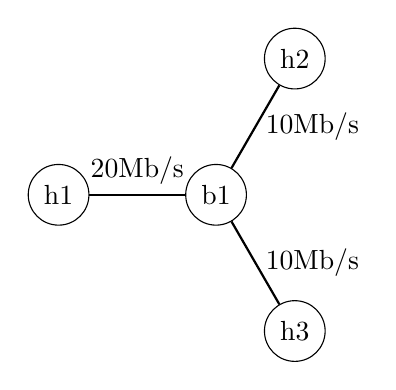
\begin{tikzpicture}[scale=1, transform shape]

% 定义节点
\node[draw, circle] (h1) at (0, 0) {h1};
\node[draw, circle] (b1) at (2, 0) {b1};
\node[draw, circle] (h2) at (3, 1.73) {h2};
\node[draw, circle] (h3) at (3, -1.73) {h3};

% 连接节点
\draw[-, thick] (h1) -- node[midway, above] {20Mb/s} (b1);
\draw[-, thick] (h2) -- node[midway, right] {10Mb/s} (b1);
\draw[-, thick] (h3) -- node[midway, right] {10Mb/s} (b1);

\end{tikzpicture}
\caption{广播网络拓扑结构}
\label{fig:hub_topo}
\end{figure}

要进行iperf测试：
\begin{enumerate}
    \item H1: iperf client; H2, H3: iperf servers
    \item H1: iperf server; H2, H3: iperf clients
\end{enumerate}
我们可以直接修改three_nodes_bw.py脚本,在启动mininet分别在h1, h2, h3节点上运行client或server程序,然后观察iperf的测试结果。
实验结果如图\ref{fig:hub_iperf}所示。
\begin{figure}[H]
  \centering
  \includegraphics[width=0.8\textwidth]{fig/hub_iperf_h1_to_h2.png}
  \includegraphics[width=0.8\textwidth]{fig/hub_iperf_h1_to_h3.png}
  \includegraphics[width=0.8\textwidth]{fig/hub_iperf_h2_to_h1.png}
  \includegraphics[width=0.8\textwidth]{fig/hub_iperf_h3_to_h1.png}
  \caption{hub广播网络iperf测试结果}
  \label{fig:hub_iperf}
\end{figure}

从实验结果可以看出，以h1为server时，h1到h2的带宽约为7.48Mbits/sec，h1到h3的带宽约为7.26 Mbits/sec，总带宽约为14.74Mbits/sec，带宽利用率约为73.7\%。
以h1为client时，h2到h1的带宽约为2.64 Mbits/sec，h3到h1的带宽约为6.16 Mbits/sec，总带宽约为8.8 Mbits/sec，带宽利用率约为44\%。
可见，h1为client时，所有数据从 h1 单一口轮流发往 h2/h3；两端返回的 TCP ACK 与数据同处一个冲突域，碰撞更频繁；
且 Hub 会把发给 h2 的帧也给到 h3 链路（反之亦然），有效带宽被“重复占用”。

\subsubsection{构建环形拓扑，验证该拓扑下节点广播会产生数据包环路}
下图\ref{fig:hub_ring_topo}为环形拓扑结构图。

\begin{figure}[H]
\centering
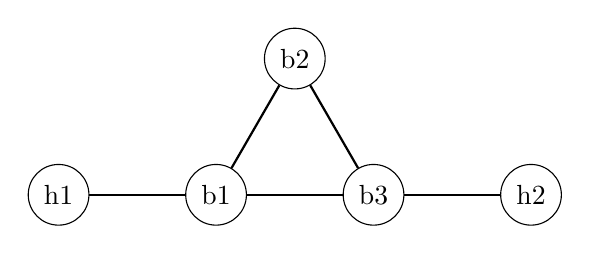
\begin{tikzpicture}[scale=1, transform shape]

% 定义节点
\node[draw, circle] (h1) at (0, 0) {h1};
\node[draw, circle] (b1) at (2, 0) {b1};
\node[draw, circle] (b2) at (3, 1.73) {b2};
\node[draw, circle] (b3) at (4, 0) {b3};
\node[draw, circle] (h2) at (6, 0) {h2};

% 连接节点
\draw[-, thick] (h1) -- (b1);
\draw[-, thick] (b1) -- (b2);
\draw[-, thick] (b2) -- (b3);
\draw[-, thick] (b3) -- (h2);
\draw[-, thick] (b3) -- (b1);

\end{tikzpicture}
\caption{广播网络拓扑结构}
\label{fig:hub_ring_topo}
\end{figure}

在该拓扑结构中，b1, b2, b3节点均作为hub连接h1, h2节点，形成环形拓扑结构。在b1, b2, b3节点运行hub程序，使用ping命令由h1向h2发送一个数据包。
通过tcpdump抓包，利用wireshark分析数据包，可以看到数据包在环形拓扑中不断循环转发，形成数据包环路，验证了环形拓扑下节点广播会产生数据包环路的现象，如图\ref{fig:hub_ring_loop}所示。

\begin{figure}[H]
  \centering
  \includegraphics[width=0.8\textwidth]{fig/hub_ring_loop_1.png}
  \includegraphics[width=0.8\textwidth]{fig/hub_ring_loop_2.png}
  \caption{环形拓扑数据包环路现象}
  \label{fig:hub_ring_loop}
\end{figure}

\subsection{实验二：交换机转发实验(switch)}
\subsubsection{交换机转发逻辑实现}

\begin{lstlisting}[language=C]
// mac.c
// lookup the mac address in mac_port table
iface_info_t *lookup_port(u8 mac[ETH_ALEN])
{
	// TODO: implement the lookup process here
	// fprintf(stdout, "TODO: implement the lookup process here.\n");
	u8 hash = hash8((char *)mac, ETH_ALEN);

	pthread_mutex_lock(&mac_port_map.lock);
	mac_port_entry_t *entry = NULL;
	list_for_each_entry(entry, &mac_port_map.hash_table[hash], list) {
		if (memcmp(entry->mac, mac, ETH_ALEN) == 0) {
			entry->visited = time(NULL);
			pthread_mutex_unlock(&mac_port_map.lock);
			return entry->iface;
		}
	}
	pthread_mutex_unlock(&mac_port_map.lock);

	return NULL;
}
...
// insert the mac -> iface mapping into mac_port table
void insert_mac_port(u8 mac[ETH_ALEN], iface_info_t *iface)
{
	// TODO: implement the insertion process here
	// fprintf(stdout, "TODO: implement the insertion process here.\n");
	u8 hash = hash8((char *)mac, ETH_ALEN);
	pthread_mutex_lock(&mac_port_map.lock);
	mac_port_entry_t *entry = NULL;
	list_for_each_entry(entry, &mac_port_map.hash_table[hash], list) {
		if (memcmp(entry->mac, mac, ETH_ALEN) == 0) {
			entry->iface = iface;
			entry->visited = time(NULL);
			pthread_mutex_unlock(&mac_port_map.lock);
			return;
		}
	}

	entry = (mac_port_entry_t *)malloc(sizeof(mac_port_entry_t));
	memcpy(entry->mac, mac, ETH_ALEN);
	entry->iface = iface;
	entry->visited = time(NULL);

	list_add_head(&entry->list, &mac_port_map.hash_table[hash]);
	pthread_mutex_unlock(&mac_port_map.lock);
}
...
// sweeping mac_port table, remove the entry which has not been visited in the
// last 30 seconds.
int sweep_aged_mac_port_entry()
{
	// TODO: implement the sweeping process here
	// fprintf(stdout, "TODO: implement the sweeping process here.\n");
	int cnt = 0;
	time_t now = time(NULL);
	pthread_mutex_lock(&mac_port_map.lock);
	mac_port_entry_t *entry, *q;
	for (int i = 0; i < HASH_8BITS; i++) {
		list_for_each_entry_safe(entry, q, &mac_port_map.hash_table[i], list) {
			if (now - entry->visited > MAC_PORT_TIMEOUT) {
				list_delete_entry(&entry->list);
				free(entry);
				cnt++;
			}
		}
	}
	pthread_mutex_unlock(&mac_port_map.lock);
	return cnt;
}

// main.c
void handle_packet(iface_info_t *iface, char *packet, int len)
{
	// TODO: implement the packet forwarding process here
	// fprintf(stdout, "TODO: implement the packet forwarding process here.\n");

	struct ether_header *eh = (struct ether_header *)packet;
	// log(DEBUG, "the dst mac address is " ETHER_STRING ".\n", ETHER_FMT(eh->ether_dhost));

	iface_info_t *dst_iface = lookup_port(eh->ether_dhost);
	if (dst_iface) {
		iface_send_packet(dst_iface, packet, len);
	} else {
		broadcast_packet(iface, packet, len);
	}

	insert_mac_port(eh->ether_shost, iface);

	free(packet);
}
\end{lstlisting}

关键代码解释：
\begin{itemize}
    \item lookup\_port函数：在mac\_port表中查找目标MAC地址对应的接口信息。如果找到则返回对应的接口信息，并更新该条目的访问时间；如果未找到则返回NULL。
    \item insert\_mac\_port函数：将MAC地址与接口信息的映射插入到mac\_port表中。如果该MAC地址已经存在，则更新对应的接口信息和访问时间；如果不存在，则创建一个新的条目并插入到表中。
    \item sweep\_aged\_mac\_port\_entry函数：遍历mac\_port表，删除那些在过去30秒内未被访问的条目，以防止表项过多导致内存浪费。
    \item handle\_packet函数：处理收到的数据包。首先查找目标MAC地址对应的接口信息，如果找到则将数据包发送到该接口；如果未找到则广播数据包。最后将源MAC地址与接收接口的信息插入到mac\_port表中。
\end{itemize}

\subsubsection{使用iperf和给定的拓扑进行实验，对比交换机转发与集线器广播的性能}
使用与实验一相同的拓扑结构，只需将hub程序替换为switch程序即可。实验结果如图\ref{fig:switch_iperf}所示。
\begin{figure}[H]
  \centering
  \includegraphics[width=0.8\textwidth]{fig/switch_iperf_h1_to_h2.png}
  \includegraphics[width=0.8\textwidth]{fig/switch_iperf_h1_to_h3.png}
  \includegraphics[width=0.8\textwidth]{fig/switch_iperf_h2_to_h1.png}
  \includegraphics[width=0.8\textwidth]{fig/switch_iperf_h3_to_h1.png}
  \caption{switch交换机转发网络iperf测试结果}
  \label{fig:switch_iperf}
\end{figure}

从实验结果可以看出，以h1为server时，h1到h2的带宽约为8.53Mbits/sec，h1到h3的带宽约为8.30 Mbits/sec，总带宽约为16.83Mbits/sec，带宽利用率约为84.15\%。
以h1为client时，h2到h1的带宽约为9.29 Mbits/sec，h3到h1的带宽约为9.19 Mbits/sec，总带宽约为18.48 Mbits/sec，带宽利用率约为92.4\%。
可见，交换机转发能够有效避免广播风暴和数据包环路问题，提高链路利用效率。这是因为交换机能够根据地址表进行有针对性的转发，而不是简单地广播数据包到所有接口。可以提高
链路利用效率，减少冲突和碰撞的发生。

\section{实验遇到的问题}
\subsection{log, printf输出导致丢包}
在实验过程中，发现框架种存在大量的DEBUG级别的log, printf输出，如果这些输出输出到终端，会严重影响程序的性能，导致ping不通, iperf测试结果异常的低。
解决方法是将这些输出重定向到文件中，或者直接注释掉这些输出语句，这样运行过程就恢复了正常。推测是因为大量的输出操作占用了过多的CPU时间，导致程序无法及时处理网络数据包，从而引发丢包现象。
\end{document}